\begin{flushright} {\tiny {\color{gray} mms\_dobo.tex}} \end{flushright}
%~~~~~~~~~~~~~~~~~~~~~~~~~~~~~~~~~~~~~~~~~~~~~~~~~~~~~~~~~~~~~~~~~~~~~~~~~~~~~~~~~~~~~~~~~~~~~~~~~~

Taken from Dohrmann \& Bochev (2004,2006) \cite{dobo04,bodg06}. 
This benchmark is also used in Worthen \etal \cite{wosp14} and Lamichhane \etal \cite{lami17}.
It is for a unit square with $\nu=\eta/\rho=1$ and the smooth exact solution is
\begin{eqnarray}
u(x,y) &=& x+x^2 - 2xy+x^3 - 3xy^2 + x^2y \\
v(x,y) &=& -y-2xy+y^2 -3x^2y + y^3 - xy^2 \\
p(x,y) &=& xy+x+y+x^3y^2 - 4/3
\end{eqnarray}
Note that the pressure field is such that $\int_{\Omega} p \; dV = 0$.
The gradient components of the velocity and pressure fields are given by:
\begin{eqnarray}
\frac{\partial u}{\partial x} &=& 3x^2+2x(y+1)-3y^2-2y+1  \nn \\
\frac{\partial u}{\partial y} &=& x(x-6y-2) \nn\\
\frac{\partial v}{\partial x} &=& -y(6x+y+2) \nn\\
\frac{\partial v}{\partial y} &=& -3x^2-2x(y+1)+3y^2+2y-1 \nn\\
\frac{\partial p}{\partial x} &=& 3x^2y^2 + y +1 \nn\\ 
\frac{\partial p}{\partial y} &=& 2x^3y+x+1 \nn
\end{eqnarray}
so that the strain rate tensor components are 
\begin{eqnarray}
\dot{\varepsilon}_{xx} &=&  3x^2+2x(y+1)-3y^2-2y+1 \\
\dot{\varepsilon}_{yy} &=& -3x^2-2x(y+1)+3y^2+2y-1 \\
\dot{\varepsilon}_{xy} &=&  \frac{1}{2} [x(x-6y-2) -y(6x+y+2) ] \\
&=& \frac{1}{2}( x^2 -y^2 -12xy -2x -2y)
\end{eqnarray}
We have
\begin{eqnarray}
\frac{\partial \dot{\varepsilon}_{xx}}{\partial x} &=& 2(3x+y+1) \\
\frac{\partial \dot{\varepsilon}_{xy}}{\partial y} &=& -6x-y-1  \\
\frac{\partial \dot{\varepsilon}_{xy}}{\partial x} &=&  -6y+x-1 \\  
\frac{\partial \dot{\varepsilon}_{yy}}{\partial y} &=& 2(3y-x+1) 
\end{eqnarray}
so that the corresponding body force is given by:
\begin{eqnarray}
b_x 
&=& \frac{\partial p}{\partial x}  
-2\frac{\partial \dot{\varepsilon}_{xx}}{\partial x} -  2\frac{\partial \dot{\varepsilon}_{xy}}{\partial y} \nn\\
&=& 3x^2y^2 + y +1  - 4(3x+y+1) - 2(-6x-y-1) \nn\\
&=& 3x^2y^2 -y-1   \\
b_y 
&=& \frac{\partial p}{\partial y} 
-2 \frac{\partial \dot{\varepsilon}_{xy}}{\partial x} - 2\frac{\partial \dot{\varepsilon}_{yy}}{\partial y}  \nn\\
&=& 2x^3y+x+1  -2(-6y+x-1) - 4(3y-x+1) \nn\\
&=& 2x^3y+3x-1 
\end{eqnarray}

Finally we have
\[
\int_0^1 \int_0^1 u^2 dxdy=
\int_0^1 \int_0^1 ( x+x^2 - 2xy+x^3 - 3xy^2 + x^2y  )^2 dx dy = \frac{401}{504} 
\]
\[
\int_0^1 \int_0^1 v^2 dxdy=
\int_0^1 \int_0^1 (-y-2xy+y^2 -3x^2y + y^3 - xy^2  )^2 dx dy = \frac{5911}{2520}
\]
so the root mean square velocity is
\[
v_{rms} = \sqrt{ \frac{1}{L_x L_y}  \int_0^1 \int_0^1 (u^2+v^2) dx dy }  
= \sqrt{\frac{401\cdot 5 + 5911}{2520}}\simeq 1.77236278... 
\]


\begin{center}
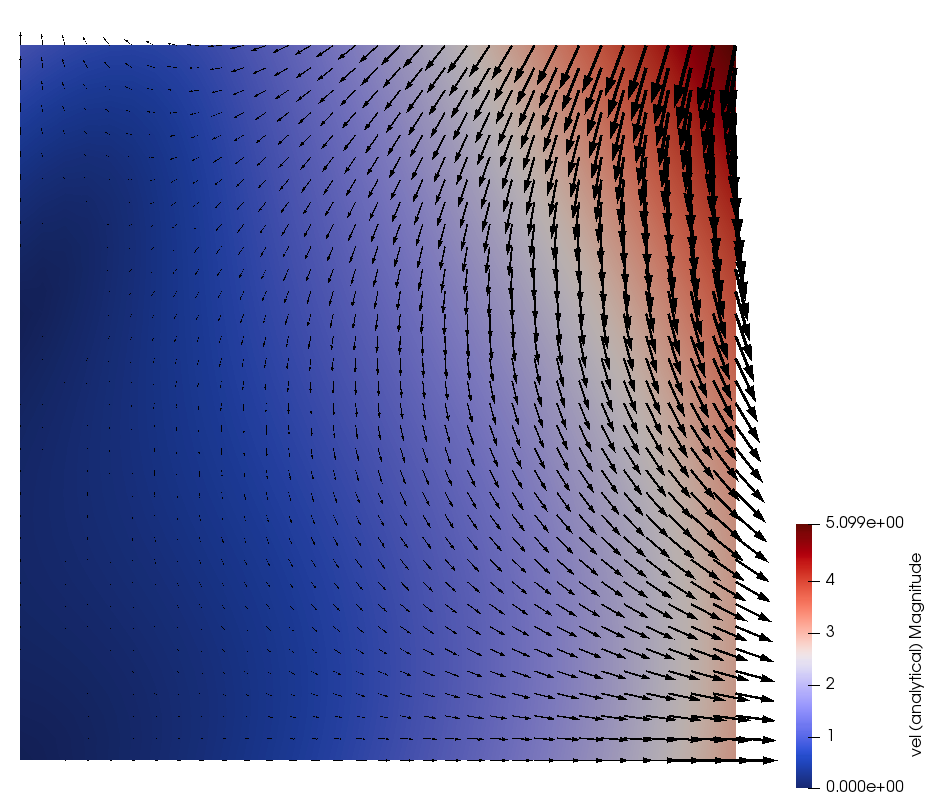
\includegraphics[width=5cm]{images/benchmark_db2d/vel}
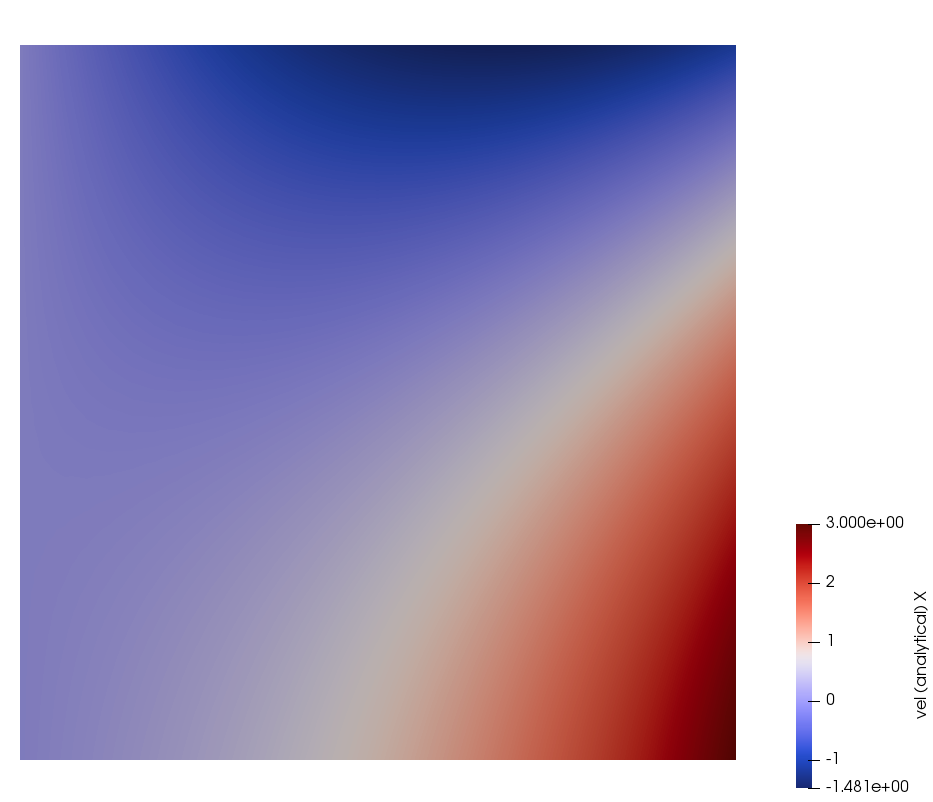
\includegraphics[width=5cm]{images/benchmark_db2d/u}
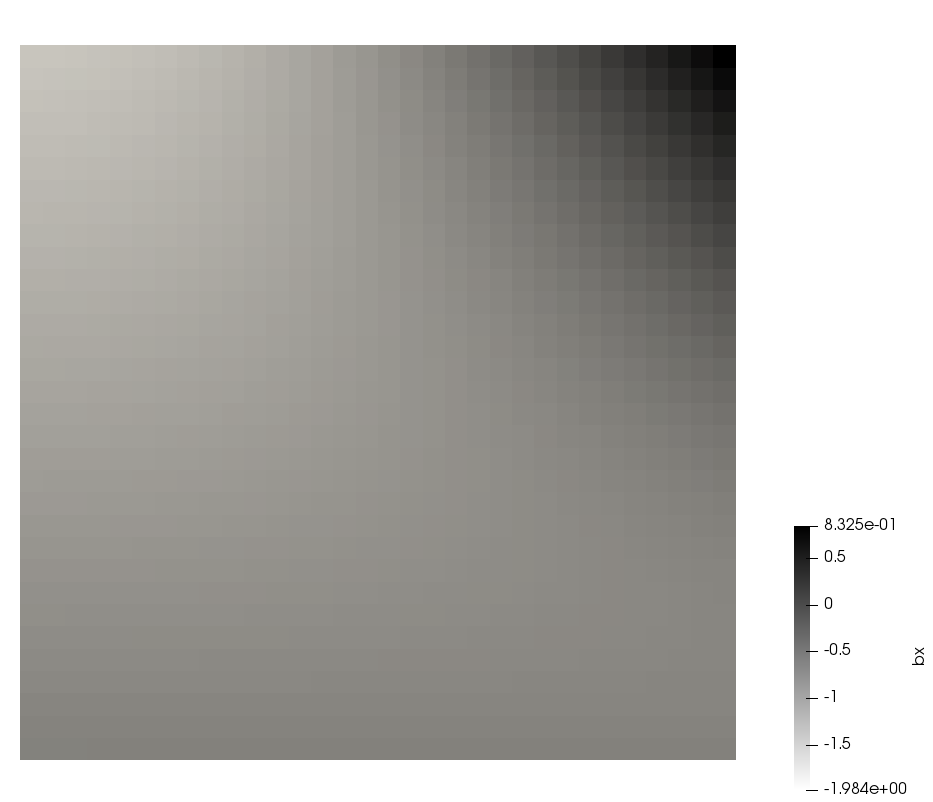
\includegraphics[width=5cm]{images/benchmark_db2d/bx}\\
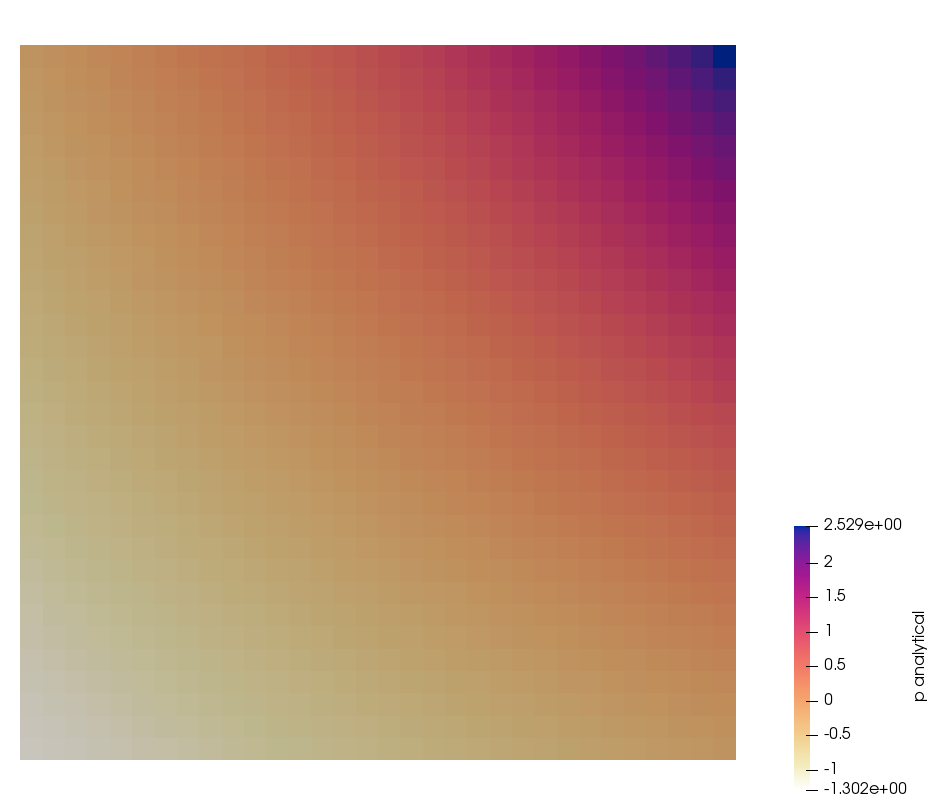
\includegraphics[width=5cm]{images/benchmark_db2d/press}
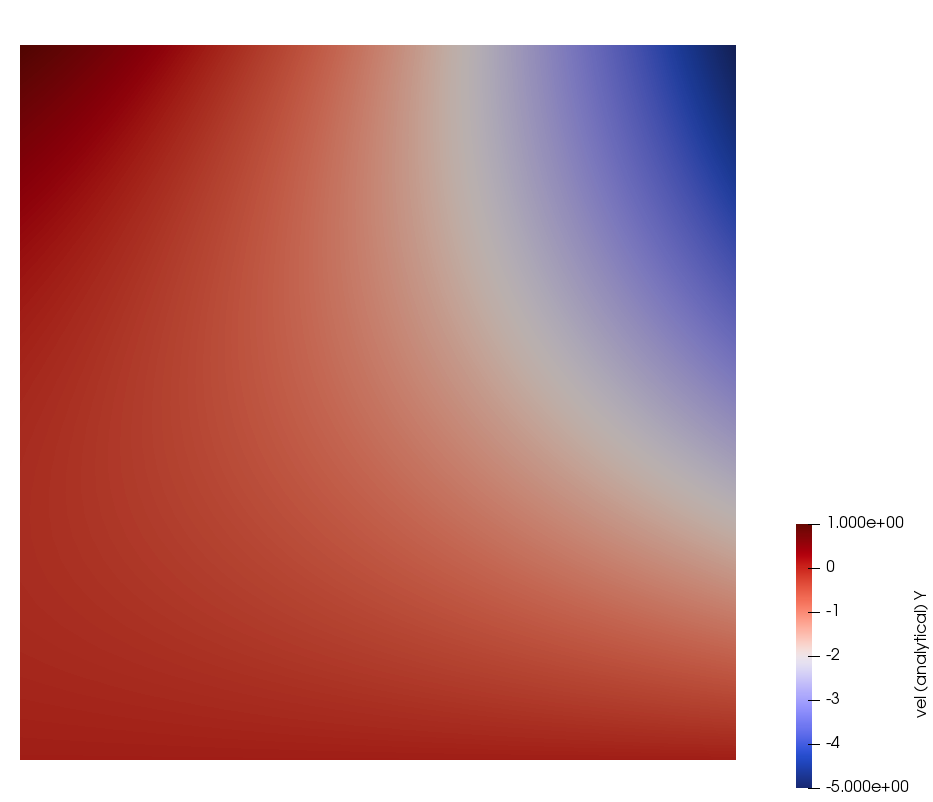
\includegraphics[width=5cm]{images/benchmark_db2d/v}
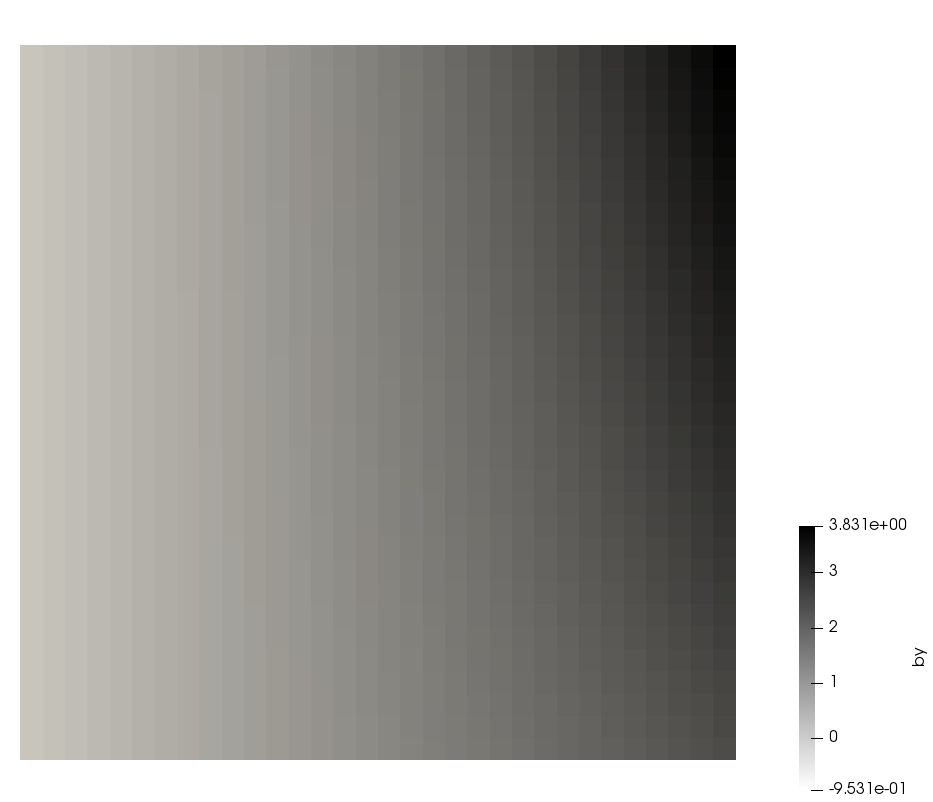
\includegraphics[width=5cm]{images/benchmark_db2d/by}
\end{center}

